\begin{frame}{Structure}
  \tableofcontents
\end{frame}

\section{Neural network ~\newline basics}

\begin{frame}{Neural network}
  \begin{definition}
    (Neural Network)
    A neural network $\Phi$ is a composition of one or multiple layers $\phi$ 
    with compatible input and ouput dimensions:
    \begin{equation*}
      \Phi(x;\Theta) = \phi_{n_L} \lb \phi_{n_L-1} \lb \cdots
      \lb \phi_2(
      \phi_1(x;\theta_1); \theta_2 ) \cdots \rb ; \theta_{n_L-1} \rb ; \theta_{n_L} \rb
    \end{equation*}
    We denote the vector of
    \bemph{all layer parameters} with $\Theta = (\theta_1^T, \dots, \theta_{n_L}^T)^T$.
  \end{definition}
  
  Example: (fully-connected) linear layer
  \begin{equation*}
    \phi(x) = Wx +b
  \end{equation*}
  with parameters $W \in \R^{n_2 \times n_1}$ 
  and $b \in \R^{n_2}$,\\
  i.e. $\theta = (vec(W)^T, b^T)^T \in \R^{n_2 n_1 + n_2}$.
\end{frame}

\begin{frame}{Training data and loss}
  Here: supervised learning

  \begin{block}{Training data}
    $\mathcal{T} = \{(x_1, y_1) \dots, (x_{n_{\text{train}}},y_{n_{\text{train}}}) \}
   \subset \R^{n_x} \times \R^{n_y}$
  \end{block}

  \begin{block}{Mini-batches}
    disjoint subsets $\mathcal{B}_1, \dots, \mathcal{B}_{n_{\text{b}}}$
    with $\mathcal{T} = \mathcal{B}_1 \cup \cdots \cup \mathcal{B}_{n_{\text{b}}}$
  \end{block}

  \begin{block}{Loss}
    \begin{equation*}
      L(\mathcal{B}; \Theta) = \sum_{(x_i,y_i) \in \mathcal{B}} l(\Phi(x_i; \Theta), y_i),
    \end{equation*}
    where $l : \R^{n_y} \times \R^{n_y} \to \R$ gives the loss for an 
    individual training sample.
  \end{block} 
\end{frame}

\begin{frame}{Gradient descent}
  learning rate $\gamma \in  \R$

  epoch $i \in \N$
  \begin{block}{Gradient descent}
    \begin{equation*}
      \Theta_{i+1} = \Theta_i - \gamma \grad[\Theta]{L(\mathcal{T};\Theta_{i})}
    \end{equation*}
  \end{block}

  If the training data is split into mini-batches:
  \begin{block}{Stochastic Gradient descent}
    \begin{equation*}
      \Theta_{i+1} = \Theta_i - \gamma \grad[\Theta]{L(
        \mathcal{B}_{((i \textrm{ mod } n_{\text{b}}) + 1)};
        \Theta_{i})}
    \end{equation*}
  \end{block}

  different gradient descent flavors, for example Adam, ...
\end{frame}

\section{Hamiltonian Systems}

\begin{frame}{Hamiltonian system}
  \begin{equation*}
    J := \begin{pmatrix}
      0 & I_d \\
      -I_d & 0
    \end{pmatrix}, \,
    d \in \N
  \end{equation*}

  \begin{definition}
    A \bemph{Hamiltonian (ODE) system} can be written in canonical form as
    \begin{align*}
      \dot{y}(t) &= J \grad{H}(y(t)) \quad \text{for } t \in I \subset \mathbb{R} \\
      y(t_0) &= y_0
      ,
    \end{align*}
    where $y: I \subset \mathbb{R} \to \mathbb{R}^{2d},\, t \mapsto y(t) = (q(t),p(t))$ and 
    $y_0 = (q_0, p_0) \in \mathbb{R}^{2d}$ the initial value at $t_0 \in I$.
    The function $H: \mathbb{R}^{2d} \to \mathbb{R}$ is called the \bemph{Hamiltonian}
    or the \bemph{total energy}. The entries of $q = q(t) \in \mathbb{R}^d$ are called 
    \bemph{generalized coordinates}
    and the entries of $p=p(t) \in \mathbb{R}^d$ are called \bemph{conjugate momenta}. 
    The \bemph{phase space} $\mathcal{V} = \mathbb{R}^{2d}$ has even dimension for Hamiltonian systems.
  \end{definition}
\end{frame}

\begin{frame}[c]{Conservation of the total energy}
  \centering
  \begin{equation*}
    \ddt H(y(t)) = \lsb \grad{H}(y(t)) \rsb^T \dot{y}(t) = 
    \lsb \grad{H}(y(t)) \rsb^T J \grad{H}(y(t)) = 0
  \end{equation*}
\end{frame}

\begin{frame}{Flow}
  flow of a Hamiltonian system
  \begin{equation*}
    \phi_{t,H}\begin{pmatrix}
      q_0 \\
      p_0
    \end{pmatrix}
    = \begin{pmatrix}
      q(t; q_0, p_0) \\
      p(t; q_0, p_0)
    \end{pmatrix}
  \end{equation*}

  \begin{definition}
    A differentiable map $\phi : U \to \mathbb{R}^{2d}$ (where $U \subset \mathbb{R}^{2d}$ is an open set)
    is called symplectic if the Jacobian matrix $\jac{\phi}{x}$ is symplectic everywhere, i.e.
    \begin{equation*}
      \lb \jac{\phi}{x} \rb^T J \lb \jac{\phi}{x} \rb = J
      .
    \end{equation*}
  \end{definition}

  \bemph{The flow $\phi_{t,H}$ of a Hamiltonian system is symplectic!} (Poincaré 1899)
\end{frame}

\section{SympNets: ~\newline Symplectic networks}

\begin{frame}[c]{Block operator}
  For $q,p \in \R^{d}$ and maps $f_{11}, f_{12}, f_{21}, f_{22} : \R^d \to \R^d$,
  we define the block operator as
  \begin{equation*}
    \begin{bmatrix}
      f_{11} & f_{12} \\
      f_{21} & f_{22}
    \end{bmatrix}
    \qpvec
    := \begin{pmatrix}
      f_{11}(q) + f_{12}(p) \\
      f_{21}(q) + f_{22}(p)
    \end{pmatrix} \in \R^{2d}
    .
  \end{equation*}
\end{frame}

\begin{frame}{The building block}
  \begin{definition}
    (Unit Triangular Layer) A layer $\phi : \mathbb{R}^{2d} \to \mathbb{R}^{2d}$ 
    is called a unit triangular layer with \bemph{layer transform}
    \begin{equation*}
      \layertf : \mathbb{R}^d \to \mathbb{R}^d,\, p \mapsto \layertf(p)
    \end{equation*}
    and bias parameter $b \in \R^{2d}$, if $\phi$ can be expressed as
    \begin{equation*}
      \phi_\up \qpvec = \uppersympop{\layertf} + b
      = \begin{pmatrix}
        q + \layertf(p) \\
        p
      \end{pmatrix} + b \quad \text{(upper unit triangular layer)}
    \end{equation*}
    or
    \begin{equation*}
      \phi_\low \qpvec = \lowersympop{\layertf} + b
      = \begin{pmatrix}
        q \\
        \layertf(q) + p
      \end{pmatrix} + b. \quad \text{(lower unit triangular layer)}
    \end{equation*}
  \end{definition}

  \bemph{A unit triangular layer is symplectic iff. the Jacobian of the 
  layer transfrom $\layertf$ is symmetric everywhere.}
\end{frame}

\begin{frame}[c]{Linear layers}
  The \bemph{linear layers} are given by the layer transform
  \begin{equation*}
    \layertf(p) = Sp
  \end{equation*}
  with a symmetric matrix $S \in \R^{d \times d}$ parametrized\\
  by $A \in \R^{d \times d}$ via $S=A^T+A$.
  \vspace{1cm}

  A linear layer can be expressed with matrix-vector multiplication:
  \begin{equation*}
    \phi_\up \qpvec = \begin{pmatrix}
      I & S \\
      0 & I
    \end{pmatrix} \qpvec + b
    .
  \end{equation*}
\end{frame}

\begin{frame}[c]{Activation layers}
  The \bemph{activation layers} are given by the layer transform
  \begin{equation*}
    \layertf(p) = \lb a_i \activation(p_i) \rb_{i=1}^d
  \end{equation*}

  with:
  \begin{itemize}
    \item an activation function $\activation : \R \to \R$
    \item coefficients $a \in \R^d$ 
  \end{itemize}
\end{frame}

\begin{frame}[c]{Gradient layers}
  The \bemph{gradient layers} are given by the layer transform
  \begin{equation*}
    \layertf(p) = K^T \bigg( a_j \activation \lb (Kp)_j + c_j \rb \bigg)_{j=1}^n
  \end{equation*}

  with:
  \begin{itemize}
    \item an activation function $\activation : \R \to \R$
    \item width $n \in \N$ ($n \gg d$)
    \item parameters $a,c \in \R^n$ and $K \in \R^{n \times d}$
  \end{itemize}
\end{frame}

\section{Normalization for ~\newline SympNets}

\begin{frame}[c]{Batch normalization}
  Initially proposed by \todo{REF}.
  \bemph{Goal:} Normalize layer input 
  to zero-mean and unit variance (with respect to the current mini-batch).

  \begin{algorithm}[H]
    \caption{Batch normalization transform $\eta_{\gamma, \beta}$}
    \textbf{Input:} mini batch $\mathcal{B} = \{x_1, x_2, \dots, x_{n_\mathcal{B}}\} \subset \R^n$ 
    and $x_k \in \mathcal{B}$ \\
    \textbf{Output:} $\eta_{\gamma, \beta}(x_k) \in \R^n$
    %\setstretch{1.5}
    \begin{algorithmic}
      \If{training\_mode} \Comment{Update mean and variance if training, otherwise
      keep previous values}
        \State $\displaystyle
        \mu_\mathcal{B} \gets \frac{1}{n_\mathcal{B}} \sum_{i=1}^{n_\mathcal{B}} x_i$
        \State $\displaystyle
        \sigma^2_\mathcal{B} \gets \frac{1}{n_\mathcal{B}} \sum_{i=1}^{n_\mathcal{B}} 
        (x_i - \mu_\mathcal{B})^2$
      \EndIf
      \State \Return 
      $\displaystyle \lb \frac{\gamma_j}{(\sigma^2_\mathcal{B})_j + \epsilon} 
      \lb (x_k)_j - \lb \mu_\mathcal{B} \rb_j \rb + \beta_j \rb_{j=1}^n$
      \Comment{Here, $\gamma, \beta \in \mathbb{R}^{n}$ are learnable parameters.}
    \end{algorithmic}
  \end{algorithm}
\end{frame}

\begin{frame}[c]{Normalized Activation layers}
  The \bemph{normalized activation layers} are given by the layer transform
  \begin{equation*}
		\layertf(p) = \lb a_i \activation(\overline{p}_i) \rb_{i=1}^d
		\quad \text{with } \overline{p} = \eta_{\gamma, \beta} \lb p \rb \in \R^d
	\end{equation*}

  with:
  \begin{itemize}
    \item an activation function $\activation : \R \to \R$
    \item parameters $a,\gamma, \beta \in \R^d$ 
  \end{itemize}
\end{frame}

\begin{frame}[c]{Normalized Gradient layers}
  The \bemph{normalized gradient layers} are given by the layer transform
  \begin{equation*}
		\layertf(p) = K^T \bigg( a_j \activation
		\lb \overline{p}_j \rb \bigg)_{j=1}^n
		\quad \text{with } \, \overline{p} = \eta_{\gamma, \beta} \lb Kp + c \rb \in \R^n
	\end{equation*}

  with:
  \begin{itemize}
    \item an activation function $\activation : \R \to \R$
    \item width $n \in \N$ ($n \gg d$)
    \item parameters $a,c,\gamma, \beta \in \R^n$ and $K \in \R^{n \times d}$
  \end{itemize}
\end{frame}

\section{Convolution for ~\newline SympNets}

\begin{frame}[c]{Convolution vs. Cross-correlation}
  Given two discrete functions $f,g \in \mathbb{R}^\mathbb{Z}$, 
  \bemph{convolution} is defined as 
  \begin{equation*}
    *: \mathbb{R}^{\mathbb{Z}} \times \mathbb{R}^{\mathbb{Z}} \to \mathbb{R}^{\mathbb{Z}},
    \quad (f*g)(\tau) = \sum^{\infty}_{a=-\infty} f(a) g(\tau - a)
    .
  \end{equation*}

  \bemph{Cross-correlation} is defined as
  \begin{equation*}
    \star: \mathbb{R}^{\mathbb{Z}} \times \mathbb{R}^{\mathbb{Z}} \to \mathbb{R}^{\mathbb{Z}},
    \quad (f \star g)(\tau) = \sum^{\infty}_{a=-\infty} f(a) g(\tau + a)
    .
  \end{equation*}
\end{frame}

\begin{frame}[c]{Valid cross-correlation}
  \begin{definition}[Valid cross-correlation]
    We define the valid cross-correlation of a finite-dimensional kernel $k \in \mathbb{R}^{n_k}$ and 
    a finite-dimensional input $x \in \mathbb{R}^{n_x}$ with $n_x \geq n_k$ as
    \begin{equation*}
      \star_{\text{v}} : \mathbb{R}^{n_k} \times \mathbb{R}^{n_x} \to \mathbb{R}^{n_x-n_k+1},
      \quad \star_{\text{v}}(k,x) := \mathcal{I}_{n_x-n_k+1}^{\text{inv}} (
        \mathcal{S}_{-1}( \mathcal{I}_{n_k}(k)) \star \mathcal{I}_{n_x}(x)
      )
      .
    \end{equation*}
  \end{definition}

  Example:
  $k \in \R^3$,
  $x \in \R^6$,
  $y := \star_{\text{v}}(k,x) \in \R^4$

  \vspace{0.3cm}
  \centering
  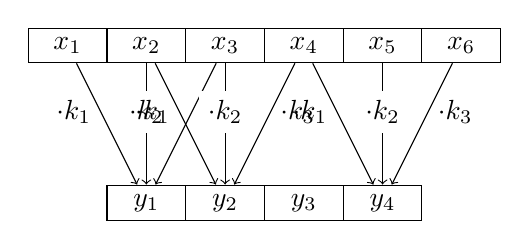
\begin{tikzpicture}
    \foreach \i in {1,2,3,4,5,6} {
      \node (x\i) [draw, minimum width=1cm] at (\i-1, 0) {$x_\i$};
    }
    \foreach \i in {1,2,3,4} {
      \node (y\i) [draw, minimum width=1cm] at (\i, -2) {$y_\i$};
    }

    \onslide<1> {
      \draw [->] (x1) edge node[left,pos=0.4]{$\cdot k_1$} (y1) ;
      \draw [->] (x2) edge node[fill=white,pos=0.4]{$\cdot k_2$} (y1);
      \draw [->] (x3) edge node[right,pos=0.4]{$\cdot k_3$} (y1);
    }

    \onslide<2> {
      \draw [->] (x2) edge node[left,pos=0.4]{$\cdot k_1$} (y2) ;
      \draw [->] (x3) edge node[fill=white,pos=0.4]{$\cdot k_2$} (y2);
      \draw [->] (x4) edge node[right,pos=0.4]{$\cdot k_3$} (y2);
    }

    \onslide<3> {
      \draw [->] (x4) edge node[left,pos=0.4]{$\cdot k_1$} (y4) ;
      \draw [->] (x5) edge node[fill=white,pos=0.4]{$\cdot k_2$} (y4);
      \draw [->] (x6) edge node[right,pos=0.4]{$\cdot k_3$} (y4);
    }
  \end{tikzpicture}
\end{frame}

\begin{frame}{Padding}
  \begin{definition}[Constant padding]
    Given the padding values $l,r \in \mathbb{R}^m$, we define constant padding 
    $c_{\text{pad},m}$ as
    \begin{equation*}
      c_{\text{pad},m} : \mathbb{R}^d \to \mathbb{R}^{d+2m},
      \quad c_{\text{pad},m}(x) = c_{\text{pad},m}(x;l,r) := \lb l^T, x^T, r^T \rb^T
      .
    \end{equation*}
  \end{definition}

  \vspace{0.3cm}
  Example:
  $l,r \in \R^3$,
  $x \in \R^6$

  \vspace{0.3cm}
  \centering
  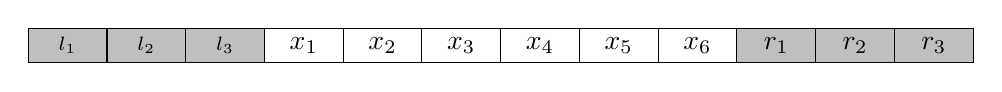
\begin{tikzpicture}
    \node [draw, minimum width=1cm,fill=lightgray] at (0, 0) {\scriptsize$l_1$};
    \node [draw, minimum width=1cm,fill=lightgray] at (1, 0) {\scriptsize$l_2$};
    \node [draw, minimum width=1cm,fill=lightgray] at (2, 0) {\scriptsize$l_3$};
    \foreach \i in {1,2,3,4,5,6} {
      \node [draw, minimum width=1cm] at (\i+2, 0) {$x_\i$};
    }
    \node [draw, minimum width=1cm,fill=lightgray] at (9, 0) {$r_1$};
    \node [draw, minimum width=1cm,fill=lightgray] at (10, 0) {$r_2$};
    \node [draw, minimum width=1cm,fill=lightgray] at (11, 0) {$r_3$};
  \end{tikzpicture}
\end{frame}

\begin{frame}{Padding}
  \begin{definition}[Symmetric padding]
    We define symmetric padding as
    \begin{equation*}
      s_{\text{pad},m} : \mathbb{R}^d \to \mathbb{R}^{d+2m},
      \quad s_{\text{pad},m}(x) := (
        \underbrace{x_m, x_{m-1} \dots, x_1}_{m \text{ values}}, \,
        \underbrace{x_1, x_2 \dots, x_d}_{d \text{ values}}, \,
        \underbrace{x_d, x_{d-1} \dots, x_{d-m+1}}_{m \text{ values}}
      )^T
      .
    \end{equation*}
  \end{definition}

  \vspace{0.3cm}
  Example:
  $x \in \R^6$

  \vspace{0.3cm}
  \centering
  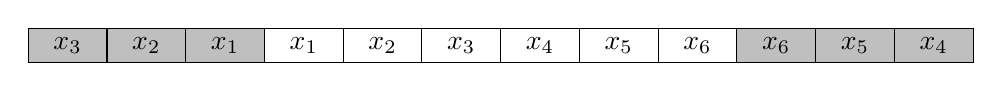
\begin{tikzpicture}
    \node [draw, minimum width=1cm,fill=lightgray] at (0, 0) {$x_3$};
    \node [draw, minimum width=1cm,fill=lightgray] at (1, 0) {$x_2$};
    \node [draw, minimum width=1cm,fill=lightgray] at (2, 0) {$x_1$};
    \foreach \i in {1,2,3,4,5,6} {
      \node [draw, minimum width=1cm] at (\i+2, 0) {$x_\i$};
    }
    \node [draw, minimum width=1cm,fill=lightgray] at (9, 0) {$x_6$};
    \node [draw, minimum width=1cm,fill=lightgray] at (10, 0) {$x_5$};
    \node [draw, minimum width=1cm,fill=lightgray] at (11, 0) {$x_4$};
  \end{tikzpicture}
\end{frame}

\begin{frame}{Symmetric kernel}
  Given an odd kernel $k \in \mathbb{R}^{2m+1}$, we set
  \begin{equation*}
    \hat{k} = \hat{k}(k) := \mathcal{S}_{-m-1}(\mathcal{I}_{2m+1}(k))
    .
  \end{equation*}
  Then $\hat{k}(-m) = k_1, \, \dots,\, \hat{k}(m) = k_{2m+1}$ and
  $\hat{k}(\tau)=0$ for $\abs{\tau} > m$.
  \begin{definition}[Symmetric kernel]
    We call an odd kernel $k \in \mathbb{R}^{2m+1}$ symmetric if
    \begin{equation*}
      \hat{k}(\tau) = \hat{k}(-\tau)
    \end{equation*}
    for all $\tau \in \mathbb{Z}$.
  \end{definition}

  For example, $k = (a,b,c,b,a) \in \R^5$ is a symmetric kernel.
\end{frame}

\begin{frame}{Parametrization of a symmetric kernel}
  Let $\{b_1, b_2, \dots b_{m+1} \} \subset \mathbb{R}^{2m+1}$ be a basis of the space 
  $\{ k \in \mathbb{R}^{2m+1} : k \text{ is a symmetric kernel} \}$.
  The symmetric kernel $k$ is then parametrized by the coefficients $\beta \in \mathbb{R}^{m+1}$ via
  \begin{equation*}
    k = (b_1, b_2, \dots, b_{m+1}) \beta = \beta_1 b_1 + \beta_2 b_2 + \dots + \beta_{m+1} b_{m+1}
    .
  \end{equation*}

  \bemph{Possible basis choices:}
  \vspace{0.3cm}
  \begin{columns}
    \column{.45\textwidth}
    \centering
    Canonical basis
    \begin{align*}
      b_1^{FD} = (\dots, 0,& 1,0, \dots)^T \in \mathbb{R}^{2m+1},\\
      b_2^{FD} = (\dots, 0, 1,&0,1, 0, \dots)^T \in \mathbb{R}^{2m+1},\\
      b_3^{FD} = (\dots, 0, 1,0,& 0,0,1, 0, \dots)^T \in \mathbb{R}^{2m+1} \\
      &\vdots
    \end{align*}

    \column{.45\textwidth}
    \centering
    Finite-difference inspired basis
    \begin{align*}
      b_1^{FD} = (\dots, 0,& 1,0, \dots)^T \in \mathbb{R}^{2m+1},\\
      b_2^{FD} = (\dots, 0, 1,-&2,1, 0, \dots)^T \in \mathbb{R}^{2m+1},\\
      b_3^{FD} = (\dots, 0, 1,-4,& 6,-4,1, 0, \dots)^T \in \mathbb{R}^{2m+1} \\
      &\vdots
    \end{align*}
  \end{columns}
\end{frame}

\begin{frame}[c]{Convolution layers}
  The (symplectic) \bemph{convolution layers} are given by the layer transform
  \begin{equation*}
    \layertf(p) := \star_{\text{v}}(k,\chi_{\text{pad},m}(p))
  \end{equation*}

  with:
  \begin{itemize}
    \item a symmetric kernel $k \in \R^{2m+1}$, 
    parametrized by $m+1$ learnable parameters
    \item padding
    $\chi_{\text{pad},m} = c_{\text{pad},m}$ or $\chi_{\text{pad},m} = s_{\text{pad},m}$
  \end{itemize}
\end{frame}

\begin{frame}{Valid cross-correlation with stride}
  Like valid cross-correlation as defined before,\\
  but skip every $s$-th output entry
  for a stride number $s \in \N$.

  \vspace{0.6cm}
  Example:
  $k \in \R^3$,
  $x \in \R^6$,
  $y := \star_{\text{v}}(k,x) \in \R^4$ with stride $s=3$

  \vspace{0.3cm}
  \centering
  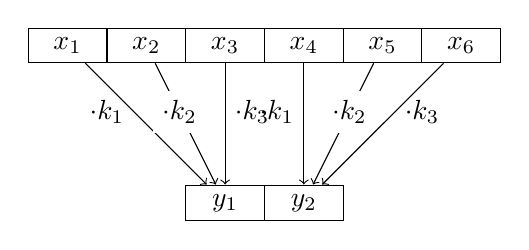
\begin{tikzpicture}
    \foreach \i in {1,2,3,4,5,6} {
      \node (x\i) [draw, minimum width=1cm] at (\i-2, 0) {$x_\i$};
    }
    \foreach \i in {1,2} {
      \node (y\i) [draw, minimum width=1cm] at (\i, -2) {$y_\i$};
    }

    \onslide<1> {
      \draw [->] (x1) edge node[left,pos=0.4]{$\cdot k_1$} (y1) ;
      \draw [->] (x2) edge node[fill=white,pos=0.4]{$\cdot k_2$} (y1);
      \draw [->] (x3) edge node[right,pos=0.4]{$\cdot k_3$} (y1);
    }

    \onslide<2> {
      \draw [->] (x4) edge node[left,pos=0.4]{$\cdot k_1$} (y2) ;
      \draw [->] (x5) edge node[fill=white,pos=0.4]{$\cdot k_2$} (y2);
      \draw [->] (x6) edge node[right,pos=0.4]{$\cdot k_3$} (y2);
    }
  \end{tikzpicture}
\end{frame}

\begin{frame}[c]{Transposed valid cross-correlation}
  \begin{itemize}
    \item For a fixed kernel $k$, valid cross-correlation (with or without stride) 
    is a linear map regarding the second argument. 
    \item Therefore there exists a representation matrix $A_{k}$ with 
    $\star_{\text{v}}(k,p) = A_{k}p$.
    \item \bemph{Transposed valid cross-correlation}
    is defined as the linear map associated with the transpose $A_{k}^T$ of $A_{k}$.
    \item We denote the transposed valid cross-correlation by $\star_{\text{v}}^T$.
  \end{itemize}
\end{frame}

\begin{frame}[c]{Convolution Gradient layers}
  The (symplectic) \bemph{convolution gradient layers} are given by the layer transform
  \begin{equation*}
    \layertf(p) = \star_{\text{v}} \lb k, \, 
    \lb a_j \activation \lb \lb \star_{\text{v}}^T(k,p) \rb_j + c_j \rb \rb_{j=1}^n \rb,
		\quad c = \star_{\text{v}}^T(\tilde{c},1_d) 
		\text{ and } a = \star_{\text{v}}^T(\tilde{a},1_d)
  \end{equation*}

  with:
  \begin{itemize}
    \item activation function $\activation : \R \to \R$
    \item kernel size $n_k \in \N$
    \item stride number $s \in N$
    \item kernel parameters $k,\tilde{a},\tilde{c} \in \R^{n_k}$
  \end{itemize}

  Here, $n \in \N$ refers to the output dimension of the
  transposed valid cross-correlation.
\end{frame}

\section{Numerical experiments}

\begin{frame}{Experiment setup}
  Given some phase space samples $x_1, \dots, x_n \in \mathcal{V}$, we generate data samples 
  \begin{equation*}
    \mathcal{T} = \{ (x_i, \phi^{\text{h}}_{t,H}(x_i)) \}_{i=1}^{n}
    \subset \mathcal{V} \times \mathcal{V}
  \end{equation*}
  for fixed time $t$.

  \vspace{0.3cm}
  The data samples $\mathcal{T}$ are split into a training data set 
  $\mathcal{T}_{\text{train}}$ and test data set $\mathcal{T}_{\text{test}}$,\\
  i.e. $\mathcal{T}_{\text{train}} \cup \mathcal{T}_{\text{test}} = \mathcal{T}$
  and $\mathcal{T}_{\text{train}} \cap \mathcal{T}_{\text{test}} = \emptyset$.

  \vspace{0.6cm}
  In all our experiments, we use the mean-square error (MSE) loss defined by
  \begin{equation*}
    L(\mathcal{B}, \Theta) = \sum_{(x_i, y_i) \in \mathcal{B}} \norm{\Phi(x_i; \Theta) - y_i}^2_2
    ,
  \end{equation*}

  \bemph{Goal:} The trained neural network is used as a numerical integrator
  to predict a trajectory of the Hamiltonian ODE system given some initial values.
\end{frame}

\begin{frame}[c]{Simple Pendulum}
  For $q,p \in \R$, the Hamiltonian for the Simple Pendulum is given by
  \begin{equation*}
    H(q,p) = \frac{p^2}{2ml^2} + mgl (1-\cos(q))
    .
  \end{equation*}
  For the experiment, we choose $m=1, g=1$ and $l=1$.

  \vspace{0.6cm}
  Training and test data uniformly sampled from
  \begin{equation*}
    \mathcal{D} = [-\frac{\pi}{2}, \frac{\pi}{2}] \times [-\sqrt{2}, \sqrt{2}]
  \end{equation*}
  with fixed time $t = 0.1$,\\
  $n_{\text{train}} = 40$ and $n_{\text{test}} = 400$.
\end{frame}

\begin{frame}[c]
  \begin{figure}
    \begin{tikzpicture}[node distance=0.3cm]
      \node (c1) [draw,text width=5cm,align=center,rotate=90]
        {\textbf{Lower} Linear layer\\ $\layertf(p) = Sp$};

      \node (c2) [draw,text width=5cm,align=center,rotate=90,right=of c1.south east,anchor=north east]
        {\textbf{Upper} Linear layer};

      \node (c3) [draw,text width=5cm,align=center,rotate=90,right=of c2.south east,anchor=north east]
        {\textbf{Lower} Linear layer};

      \node (c4) [draw,text width=5cm,align=center,rotate=90,right=of c3.south east,anchor=north east]
        {\textbf{Upper} Linear layer};

      \node (lin) [fit=(c1) (c2) (c3) (c4)] {};
      \node (lin_title) [below=0cm of lin] {\bemph{Linear block}};
      \node (lin_block) [draw,fit=(lin) (lin_title)] {};

      \node (x) [left=of lin] {$x = \qpvec$};

      \node (a1) [draw,text width=5cm,align=center,rotate=90,right=of c4.south east,anchor=north east,
        yshift=-0.2cm,fill=uniSlightblue]
        {\textbf{Lower} Activation layer\\ $\layertf(p) = \lb a_i \activation(p_i) \rb_{i=1}^d$};

      \node (lin_block2) [draw,text width=5cm,align=center,rotate=90,right=of a1.south east,anchor=north east]
        {\bemph{Linear block}};

      \node (a2) [draw,text width=5cm,align=center,rotate=90,right=of lin_block2.south east,anchor=north east,
        fill=uniSlightblue]
        {\textbf{Upper} Activation layer};

      \node (lin_block3) [draw,text width=5cm,align=center,rotate=90,right=of a2.south east,anchor=north east]
        {\bemph{Linear block}};

      \node (a3) [draw,text width=5cm,align=center,rotate=90,right=of lin_block3.south east,anchor=north east,
        fill=uniSlightblue]
        {\textbf{Lower} Activation layer};

      \node (lin_block4) [draw,text width=5cm,align=center,rotate=90,right=of a3.south east,anchor=north east]
        {\bemph{Linear block}};

      \node (a4) [draw,text width=5cm,align=center,rotate=90,right=of lin_block4.south east,anchor=north east,
        fill=uniSlightblue]
        {\textbf{Upper} Activation layer};

      \node (y) [right=of a4.south] {$y$};

      \draw[->] (x) -- (c1);
      \draw[->] (c1) -- (c2);
      \draw[->] (c2) -- (c3);
      \draw[->] (c3) -- (c4);
      \draw[->] (c4) -- (a1);
      \draw[->] (a1) -- (lin_block2);
      \draw[->] (lin_block2) -- (a2);
      \draw[->] (a2) -- (lin_block3);
      \draw[->] (lin_block3) -- (a3);
      \draw[->] (a3) -- (lin_block4);
      \draw[->] (lin_block4) -- (a4);
      \draw[->] (a4) -- (y);
    \end{tikzpicture}

    \caption{\bemph{LA-SympNet architecture.} For the activation layers,\\
    $\tanh$ is used as the activation function.}
  \end{figure}
\end{frame}

\begin{frame}[c]
  \begin{figure}
    \begin{tikzpicture}[node distance=0.3cm]
      \node (g1) [draw,text width=6cm,align=center,rotate=90,fill=uniSyellow]
        {\textbf{Lower} Gradient layer (width $n=30$)\\ $\layertf(p) = K^T \bigg( a_j \activation \lb (Kp)_j + c_j \rb \bigg)_{j=1}^n$};

      \node (g2) [draw,text width=6cm,align=center,rotate=90,
        right=of g1.south east,anchor=north east,fill=uniSyellow]
        {\textbf{Upper} Gradient layer (width $n=30$)};

      \node (g3) [draw,text width=6cm,align=center,rotate=90,
        right=of g2.south east,anchor=north east,fill=uniSyellow]
        {\textbf{Lower} Gradient layer (width $n=30$)};

      \node (g4) [draw,text width=6cm,align=center,rotate=90,
        right=of g3.south east,anchor=north east,fill=uniSyellow]
        {\textbf{Upper} Gradient layer (width $n=30$)};

      \node (x) [left=of g1.north] {$x = \qpvec$};
      \node (y) [right=of g4.south] {$y$};

      \draw[->] (x) -- (g1);
      \draw[->] (g1) -- (g2);
      \draw[->] (g2) -- (g3);
      \draw[->] (g3) -- (g4);
      \draw[->] (g4) -- (y);
    \end{tikzpicture}

    \caption{\bemph{G-SympNet architecture.}
    $\tanh$ is used as the activation function.}
  \end{figure}
\end{frame}

\begin{frame}{Simple pendulum}
  \begin{tikzpicture}
    \begin{groupplot}[	
      group style={
        group size=2 by 1,
        y descriptions at=edge left,
        horizontal sep=0.1cm,
        vertical sep=2.2cm,
      },
      xlabel=Epoch, ylabel=Loss,
      width=0.9*\axisdefaultwidth, height=7cm,
      no markers,
      ymax=1e-1, ymin=5e-10, ymode=log,
      legend style={nodes={scale=0.75, transform shape}},
      legend entries={
        FNN,
        LA-SympNet,
        N1-LA-SympNet,
        G-SympNet,
        N1-G-SympNet,
      }
    ]
    \nextgroupplot[title={Training loss (tanh activation)}]
      \addplot[
        color=green
      ] table[x=epoch,y=loss,col sep=comma] {../../data/simple_pendulum_swing/fnn/tanh/loss.csv};

      \addplot[
        color=red
      ] table[x=epoch,y=loss,col sep=comma] {../../data/simple_pendulum_swing/la-sympnet/tanh/loss.csv};

      \addplot[
        color=purple, densely dashed
      ] table[x=epoch,y=loss,col sep=comma] {../../data/simple_pendulum_swing/n1-la-sympnet/tanh/loss.csv};

      \addplot[
        color=blue
      ] table[x=epoch,y=loss,col sep=comma] {../../data/simple_pendulum_swing/g-sympnet/tanh/loss.csv};

      \addplot[
        color=olive, densely dashed
      ] table[x=epoch,y=loss,col sep=comma] {../../data/simple_pendulum_swing/n1-g-sympnet/tanh/loss.csv};

    \nextgroupplot[title={Test loss (tanh activation)}]
      \addplot[
        color=green
      ] table[x=epoch,y=loss,col sep=comma] {../../data/simple_pendulum_swing/fnn/tanh/test_loss.csv};

      \addplot[
        color=red
      ] table[x=epoch,y=loss,col sep=comma] {../../data/simple_pendulum_swing/la-sympnet/tanh/test_loss.csv};

      \addplot[
        color=purple, densely dashed
      ] table[x=epoch,y=loss,col sep=comma] {../../data/simple_pendulum_swing/n1-la-sympnet/tanh/test_loss.csv};

      \addplot[
        color=blue
      ] table[x=epoch,y=loss,col sep=comma] {../../data/simple_pendulum_swing/g-sympnet/tanh/test_loss.csv};

      \addplot[
        color=olive, densely dashed
      ] table[x=epoch,y=loss,col sep=comma] {../../data/simple_pendulum_swing/n1-g-sympnet/tanh/test_loss.csv};

    \end{groupplot}
  \end{tikzpicture}
\end{frame}

\begin{frame}
  \begin{figure}
    \centering
    \begin{tikzpicture}
      \begin{groupplot}[
        group style={
          group size=2 by 1,
          horizontal sep=2cm
        },
        no markers,
        xlabel={t},
        width=0.9*\axisdefaultwidth, height=7cm,
        legend style={nodes={scale=0.75, transform shape}},
        legend entries={
          Ground truth,
          FNN (tanh),
          N1-LA-SympNet (tanh),
          N1-G-SympNet (tanh)
        }
      ]
  
      \nextgroupplot[title={Total energy $H$}, ylabel={$H(t)$}, xmin=0, xmax=100]
        \addplot[
          color=darkgray
        ] table[x=t,y=E,col sep=comma] {../../data/simple_pendulum_swing/exact/swinging_case/total_energy.csv};
  
        \addplot[
          color=green
        ] table[x=t,y=E,col sep=comma] {../../data/simple_pendulum_swing/fnn/tanh/swinging_case/total_energy.csv};
  
        \addplot[
          color=purple,densely dashed
        ] table[x=t,y=E,col sep=comma] {../../data/simple_pendulum_swing/n1-la-sympnet/tanh/swinging_case/total_energy.csv};
  
        \addplot[
          color=olive,densely dashed
        ] table[x=t,y=E,col sep=comma] {../../data/simple_pendulum_swing/n1-g-sympnet/tanh/swinging_case/total_energy.csv};
  
      \nextgroupplot[title={Predicted position $q$}, ylabel={$q(t)$}, xmin=91, xmax=97, legend pos=north west]
        \addplot[
          color=darkgray
        ] table[x=t,y=q,col sep=comma] {../../data/simple_pendulum_swing/exact/swinging_case/q.csv};
  
        \addplot[
          color=green
        ] table[x=t,y=q,col sep=comma] {../../data/simple_pendulum_swing/fnn/tanh/swinging_case/q.csv};
  
        \addplot[
          color=purple,densely dashed
        ] table[x=t,y=q,col sep=comma] {../../data/simple_pendulum_swing/n1-la-sympnet/tanh/swinging_case/q.csv};
  
        \addplot[
          color=olive,densely dashed
        ] table[x=t,y=q,col sep=comma] {../../data/simple_pendulum_swing/n1-g-sympnet/tanh/swinging_case/q.csv};
        
      \end{groupplot}
    \end{tikzpicture}
    \caption{Total energy and position over time for simple pendulum for $q_0 = \frac{\pi}{2},\, p_0 = 0$.}
  \end{figure}
\end{frame}

\begin{frame}{Semi-linear wave equation}
  One-dimensional semi-linear wave equation with constant speed $c \in \R$, nonlinear term 
  $g : \R \to \R$, domain length $l \in \R$ and domain $\Omega = [-l/2, l/2]$:
  \begin{equation*}
    \frac{\partial^2}{\partial t^2} u(t,x) = 
    c^2 \frac{\partial^2}{\partial x^2} u(t,x) - g(u(t,x)) 
    \quad \forall x \in \Omega, 
    \, t \in I \subset \R
  \end{equation*}
  Initial conditions:
  \begin{align*}
    u(t_0,x) &= u_0(x) \\
    \deldelt u(t_0,x) &= w_0(x) \quad \forall x \in \Omega
  \end{align*}
  Dirichlet boundary conditions:
  \begin{equation*}
    u(t,-l/2) = u_{\text{left}}, \, u(t,l/2) = u_{\text{right}} \quad \forall t \in I \subset \R
  \end{equation*}
\end{frame}

\begin{frame}{Semi-linear wave equation as Hamiltonian ODE}
  Given an equally-spaced grid $\{ x_i \}_{n=0}^{n+1} \subset \Omega$, $x_0 = -l/2$, $x_{n+1} = l/2$,
  with grid width $\Delta x$,\\
  initial values $y_0 = (\bar{q}_0^T, \bar{p}_0^T)^T \in \R^{2n}$, $\bar{q}_0 = \lb u_0(x_i) \rb_{i=1}^n \in \R^n$, 
  $\bar{p}_0 = \lb w_0(x_i) \rb_{i=1}^n \in \R^n$,
  the resulting \bemph{Hamiltonian system} is given by
  \begin{align*}
    \dot{y}(t) &= \frac{J_{2n}}{\Delta x} \grad{H}(y(t)) \quad \text{for } t \in I \subset \mathbb{R} \\
    y(t_0) &= y_0
  \end{align*}
  with Hamiltonian
  \begin{equation*}
    H(q,p) = \sum_{i=1}^n \Delta x \lb 
    \frac{1}{2} p_i^2 + \frac{c^2 (q_{i+1} - q_i)^2}{4 \Delta x^2} 
    + \frac{c^2 (q_i - q_{i-1})^2}{4 \Delta x^2} + G(q_i)
    \rb
    \quad (q,p \in \R^n)
    ,
  \end{equation*}
  where $G'(u) = \int_0^u g(v) dv$, $q_0 := u_{\text{left}}$ and $q_{n+1} := u_{\text{right}}$.
  The generalized coordinates $q_i(t)$ then refer to $u(t,x_i)$ and 
  the conjugate momenta $p_i(t)$ then refer to $\deldelt u(t,x_i)$.
\end{frame}

\begin{frame}[c]{Linear wave equation}
  $G(u) = g(u) =0$. We set $c=1, l=1$ and use $100$ grid points for the discretization.

  \vspace{0.3cm}
  \begin{itemize}
    \item Training and test data originate from a single trajectory and\\
    are generated with fixed time $t = 0.01$.
    \item Training data corresponds to trajectory for total time $T=0$ to $T=1$.
    \item Test data corresponds to trajectory for total time $T=1$ to $T=10$ (extrapolation).
  \end{itemize}
  
\end{frame}

\begin{frame}[c]
  \begin{figure}
    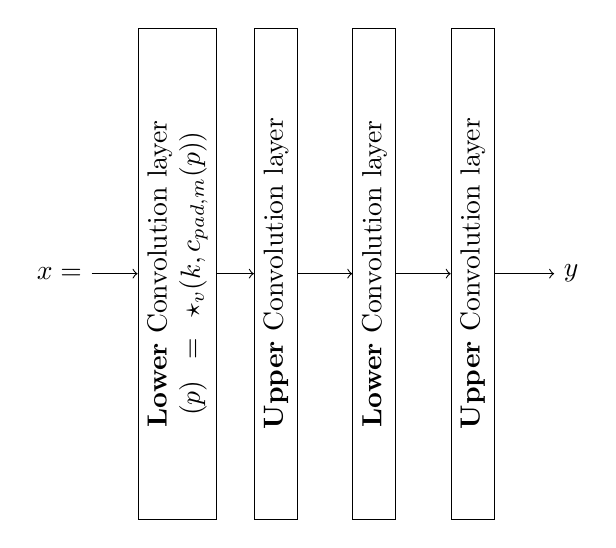
\begin{tikzpicture}
      \node (x) at (0,0) {$x = \qpvec$};

      \node (c1) [draw,text width=6cm,align=center,rotate=90] at (1.5,0) 
        {\textbf{Lower} Convolution layer\\ $\layertf(p) = \star_{\text{v}}(k,c_{\text{pad},m}(p))$};

      \node (c2) [draw,text width=6cm,align=center,rotate=90] at (2.75,0) 
        {\textbf{Upper} Convolution layer};

      \node (c3) [draw,text width=6cm,align=center,rotate=90] at (4,0) 
        {\textbf{Lower} Convolution layer};

      \node (c4) [draw,text width=6cm,align=center,rotate=90] at (5.25,0) 
        {\textbf{Upper} Convolution layer};

      \node (y) at (6.5,0) {$y$};

      \draw[->] (x) -- (c1);
      \draw[->] (c1) -- (c2);
      \draw[->] (c2) -- (c3);
      \draw[->] (c3) -- (c4);
      \draw[->] (c4) -- (y);
    \end{tikzpicture}

    \caption{\bemph{C-SympNet architecture.} 
    All layers with kernel size $3$, constant zero-padding.}
  \end{figure}
\end{frame}

\begin{frame}{Linear wave equation}
  \centering
  \begin{tikzpicture}
    \begin{axis}[
      ymode=log,
      no markers,
      title={Test loss (Linear wave equation)},
      xlabel={Epoch}, xmin=0, xmax=500,
      ylabel={Test loss},
      legend style={nodes={scale=0.75, transform shape}},
      legend cell align=left,
      legend entries={
        CNN,
        C-SympNet (canonical basis),
        C-SympNet (FD basis)
      }
    ]
  
    \addplot[
      color=green
    ] table[x=epoch,y=loss,col sep=comma] {../../data-wave/transport/linear_cnn/sigmoid/test_loss.csv};
  
    \addplot[
      color=blue
    ] table[x=epoch,y=loss,col sep=comma] {../../data-wave/transport/linear_canonical/sigmoid/test_loss.csv};
  
    \addplot[
      color=purple
    ] table[x=epoch,y=loss,col sep=comma] {../../data-wave/transport/linear_fd/sigmoid/test_loss.csv};
      
    \end{axis}
  \end{tikzpicture}
\end{frame}

\begin{frame}{Linear wave equation}
  \centering
  \begin{tikzpicture}
    \begin{axis}[
      title={Displacement $q(t=0,x)$}, ylabel={$q(t=0,x)$},
			legend entries={
				Initial value
      },
      width=0.8*\linewidth, height=\axisdefaultheight,
			xlabel={$x$}, xmin=-0.5, xmax=0.5,
			ymin=-0.3, ymax=0.55, restrict y to domain=-2:2
    ]
      \addplot[
				color=darkgray
			] table[x=x,y=q,col sep=comma] {../../data-wave/transport/exact/q_t0.csv};
    \end{axis}
  \end{tikzpicture}
\end{frame}

\begin{frame}{Linear wave equation}
  \centering
  \begin{tikzpicture}
    \begin{axis}[
      width=0.8*\linewidth, height=\axisdefaultheight,
			xlabel={$x$}, xmin=-0.5, xmax=0.5,
			ymin=-0.3, ymax=0.55, restrict y to domain=-2:2,
      title={Displacement $q(t=3,x)$}, ylabel={$q(t=3,x)$},
			legend style={
				nodes={scale=0.8, transform shape},
				legend cell align=left,
				%legend pos=outer north east
			},
			legend entries={
				CNN,
				C-SympNet (canonical basis),
				C-SympNet (FD basis),
				Ground truth,
			}
    ]
      \addplot[
        color=green
      ] table[x=x,y=q,col sep=comma] {../../data-wave/transport/linear_cnn/sigmoid/q_t3.csv};
    
      \addplot[
        color=blue
      ] table[x=x,y=q,col sep=comma] {../../data-wave/transport/linear_canonical/sigmoid/q_t3.csv};
    
      \addplot[
        color=purple
      ] table[x=x,y=q,col sep=comma] {../../data-wave/transport/linear_fd/sigmoid/q_t3.csv};

      \addplot[
        color=darkgray
      ] table[x=x,y=q,col sep=comma] {../../data-wave/transport/exact/q_t3.csv};
    \end{axis}
  \end{tikzpicture}
\end{frame}

\begin{frame}{Linear wave equation}
  \centering
  \begin{tikzpicture}
    \begin{axis}[
      width=0.8*\linewidth, height=\axisdefaultheight,
			xlabel={$x$}, xmin=-0.5, xmax=0.5,
			ymin=-0.3, ymax=0.55, restrict y to domain=-2:2,
      title={Displacement $q(t=9,x)$}, ylabel={$q(t=9,x)$},
			legend style={
				nodes={scale=0.8, transform shape},
				legend cell align=left,
				%legend pos=outer north east
			},
			legend entries={
				CNN,
				C-SympNet (canonical basis),
				C-SympNet (FD basis),
				Ground truth,
			}
    ]
      \addplot[
        color=green
      ] table[x=x,y=q,col sep=comma] {../../data-wave/transport/linear_cnn/sigmoid/q_t9.csv};
    
      \addplot[
        color=blue
      ] table[x=x,y=q,col sep=comma] {../../data-wave/transport/linear_canonical/sigmoid/q_t9.csv};
    
      \addplot[
        color=purple
      ] table[x=x,y=q,col sep=comma] {../../data-wave/transport/linear_fd/sigmoid/q_t9.csv};

      \addplot[
        color=darkgray
      ] table[x=x,y=q,col sep=comma] {../../data-wave/transport/exact/q_t9.csv};
    \end{axis}
  \end{tikzpicture}
\end{frame}

\begin{frame}[c]{Sine-Gordon}
  Semi-linear wave equation with $G(u) = 1 - \cos(u)$, $g(u) = \sin(u)$ and $c=1$.

  We use $2000$ grid points for the discretization.

  \vspace{0.3cm}
  \begin{itemize}
    \item Training and test data originate from a single trajectory and\\
    are generated with fixed time $t = 0.01$.
    \item Training data corresponds to trajectory for total time $T=0$ to $T=1$.
  \end{itemize}
\end{frame}

\begin{frame}[c]
  \begin{figure}
    \begin{tikzpicture}[node distance=0.3cm]
      \node (c1) [draw,text width=6.5cm,align=center,rotate=90]
        {\textbf{Lower} Convolution layer\\ $T(p) = \star_{\text{v}}(k,\chi_{\text{pad},m}(p))$};

      \node (g1) [draw,text width=6.5cm,align=center,rotate=90,
        right=of c1.south east,anchor=north east,fill=uniSyellow]
        {\textbf{Lower} Convolution Gradient layer\\ 
        \small$\layertf(p) = \star_{\text{v}} \lb k, \, 
        \lb a_j \activation \lb \lb \star_{\text{v}}^T(k,p) \rb_j + c_j \rb \rb_{j=1}^n \rb$};

      \node (c2) [draw,text width=6.5cm,align=center,rotate=90,
        right=of g1.south east,anchor=north east]
        {\textbf{Upper} Convolution layer};

      \node (g2) [draw,text width=6.5cm,align=center,rotate=90,
        right=of c2.south east,anchor=north east,fill=uniSyellow]
        {\textbf{Upper} Convolution Gradient layer};
      
      \node (c3) [draw,text width=6.5cm,align=center,rotate=90,
        right=of g2.south east,anchor=north east]
        {\textbf{Lower} Convolution layer};

      \node (g3) [draw,text width=6.5cm,align=center,rotate=90,
        right=of c3.south east,anchor=north east,fill=uniSyellow]
        {\textbf{Lower} Convolution Gradient layer};

      \node (c4) [draw,text width=6.5cm,align=center,rotate=90,
        right=of g3.south east,anchor=north east]
        {\textbf{Upper} Convolution layer};

      \node (g4) [draw,text width=6.5cm,align=center,rotate=90,
        right=of c4.south east,anchor=north east,fill=uniSyellow]
        {\textbf{Upper} Convolution Gradient layer};

      \node (x) [left=of c1.north] {$x = \qpvec$};
      \node (y) [right=of g4.south] {$y$};

      \draw[->] (x) -- (c1);
      \draw[->] (c1) -- (g1);
      \draw[->] (g1) -- (c2);
      \draw[->] (g2) -- (c3);
      \draw[->] (c3) -- (g3);
      \draw[->] (g3) -- (c4);
      \draw[->] (c4) -- (g4);
      \draw[->] (g4) -- (y);
    \end{tikzpicture}

    \caption{
      \bemph{CG-SympNet architecture.} Convolution layers with kernel size $3$ and FD basis.
      Convolution Gradient layers with kernel size $100$, stride $100$ and $\tanh$ activation
      function.
    }
  \end{figure}
\end{frame}

\begin{frame}{Sine-Gordon}
  \centering
  \begin{tikzpicture}
    \begin{axis}[
      width=0.8*\linewidth, height=\axisdefaultheight,
      no markers,
      xlabel={$x$}, xmin=-25, xmax=25,
			ymin=-1, ymax=10, restrict y to domain=-5:10,
      title={Displacement $q(t=0,x)$}, ylabel={$q(t=0,x)$},
			legend entries={
				Initial value
			}
    ]
      
      \addplot[
          color=darkgray
        ] table[x=x,y=q,col sep=comma] {../../data-wave/sine_gordon/exact/q_t0.csv};
      
    \end{axis}
  \end{tikzpicture}
\end{frame}

\begin{frame}{Sine-Gordon}
  \centering
  \begin{tikzpicture}
    \begin{axis}[
      width=0.8*\linewidth, height=\axisdefaultheight,
      no markers,
      xlabel={$x$}, xmin=-25, xmax=25,
			ymin=-1, ymax=10, restrict y to domain=-5:10,
      title={Displacement $q(t=3,x)$}, ylabel={$q(t=3,x)$},
			legend entries={
				CNN,
				CG-SympNet (tanh),
			  Ground truth,
			}
    ]
      
      \addplot[
        color=green
      ] table[x=x,y=q,col sep=comma] {../../data-wave/sine_gordon/cnn/elu/q_t3.csv};
    
      \addplot[
        color=red
      ] table[x=x,y=q,col sep=comma] {../../data-wave/sine_gordon/gradient/tanh/q_t3.csv};

      \addplot[
        color=darkgray
      ] table[x=x,y=q,col sep=comma] {../../data-wave/sine_gordon/exact/q_t3.csv};
      
    \end{axis}
  \end{tikzpicture}
\end{frame}

\begin{frame}{Sine-Gordon}
  \centering
  \begin{tikzpicture}
    \begin{axis}[
      width=0.8*\linewidth, height=\axisdefaultheight,
      no markers,
      xlabel={$x$}, xmin=-25, xmax=25,
			ymin=-1, ymax=10, restrict y to domain=-5:10,
      title={Displacement $q(t=9,x)$}, ylabel={$q(t=9,x)$},
			legend entries={
				CNN,
				CG-SympNet (tanh),
			  Ground truth,
			}
    ]
      
      \addplot[
        color=green
      ] table[x=x,y=q,col sep=comma] {../../data-wave/sine_gordon/cnn/elu/q_t9.csv};
    
      \addplot[
        color=red
      ] table[x=x,y=q,col sep=comma] {../../data-wave/sine_gordon/gradient/tanh/q_t9.csv};

      \addplot[
        color=darkgray
      ] table[x=x,y=q,col sep=comma] {../../data-wave/sine_gordon/exact/q_t9.csv};
      
    \end{axis}
  \end{tikzpicture}
\end{frame}

\begin{frame}{References}
  \todo{Add references}
\end{frame}